\documentclass[a4paper,12pt,brazil,doubleside]{book}

% tentei incluir o da pasta comum mas não funcionou
% \usepackage{amssymb}                        %%% para simbolo de 'marca registrada'
\usepackage[brazil]{varioref}               %%% referencias com página \vref
\usepackage[sf,bf,compact,topmarks,calcwidth,pagestyles]{titlesec} %%% definir títulos de seção
\usepackage{amsmath,amsfonts,amstext,amsthm,textcomp}
\usepackage{fancybox}                       %%% boxes
\usepackage[dvipsnames,usenames]{color}                          %%% Cores de fonte e fundo
\usepackage[dvipsnames,usenames]{xcolor}
\usepackage{colortbl}                       %%% Cores em tabelas
\usepackage{rotating}
\usepackage{fancyvrb}                       %%% Inclusão de texto usando VerbatimInput
\usepackage{bookman}                        %%% Fonte de Letras
\usepackage{enumerate}
\usepackage{lettrine}
\usepackage{minted}	
\usepackage{caption}
\usepackage{framed}
\usepackage{enumitem}

%\usepackage{listings}
%\lstset{
%  numbers=left,
%  numberstyle=\tiny,
%  mathescape=true,
%  frame=single,
%  stepnumber=1,
%%  basicstyle=\scriptsize, % fontes menores nos codigos
%  keywordstyle=\ttfamily,
%  identifierstyle=\ttfamily, % \bfseries negrito nos codigos
%  commentstyle=\ttfamily
%}
\usepackage{pstricks} % listings color: black!50!red

\usepackage{listings}
\lstset{
	numbers=left,
	stepnumber=1,
	firstnumber=1,
	numberstyle=\tiny,
	mathescape=true,
	extendedchars=true,
	breaklines=true,
	frame=single,
	basicstyle=\footnotesize,
%	basicstyle=\scriptsize,
	stringstyle=\ttfamily,
% 	moredelim=*[l][\itshape]{||},%
	showstringspaces=false,
	float=h,
}
\lstdefinelanguage{lalp} {
  sensitive=true,
  keywordstyle={\color{black!50!green}\ttfamily\bfseries},
  keywords={const, typedef, fixed, in, out, counter, when, block_ram, delay_op, mult_op_s, add_reg_op_s},
  otherkeywords={<-},
  otherkeywords={@},
  commentstyle={\color{black!50!red}\itshape},
  morecomment=[l]{//}, 
  morecomment=[s]{/*}{*/},
}
\lstdefinelanguage{ican} {
  sensitive=true,
  keywordstyle={\color{black!50!red}\ttfamily\bfseries},
  keywords={array, begin, boolean, by, case, character, default, do, each, elif, else, end, enum, esac, false, fi, for, goto, if, in, inout, integer, nil, od, of, out, procedure, real, record, repeat, return, returns, sequence, set, to, true, until, where, while},
  commentstyle={\color{black!50!green}\itshape},
  morecomment=[l]{||},
  literate={{(X)}{$\times$}1 {(E)}{$\in$}1 {(U)}{$\cup$}1 {(N)}{$\cap$}1 {(<)}{$\langle$}1 {(>)}{$\rangle$}1 {->}{$\rightarrow$}2 {<\-}{$\leftarrow$}2 {=}{$=$}1 {>}{$>$}1 {<}{$<$}1 {!=}{$\neq$}1 {>=}{$\ge$}1 {<=}{$\le$}1}
}

\renewcommand\listingscaption{Algoritmo}
\renewcommand\listoflistingscaption{Lista de Algoritmos}


\usepackage[english,brazil]{babel}
\usepackage[utf8]{inputenc}
\usepackage[T1]{fontenc}
\usepackage{times}
\usepackage{graphicx,xr}
\usepackage{subfigure}
\usepackage{longtable}
\usepackage{setspace}
\usepackage{multirow}
\usepackage{rotating}
\usepackage{indentfirst}
\usepackage{xspace}
\usepackage[sort]{natbib}
\usepackage[a4paper,top=30mm,bottom=20mm,left=30mm,right=20mm]{geometry}

\usepackage{hyperref}
\hypersetup{
%  backref, %omitir na versão final
  pdfsubject =	{...},
  pdftitle =	{...},
  pdfkeywords = {...},
  pdfauthor =	{Ricardo Menotti, Daniel Lucrédio, ...},
  colorlinks =	{true}, %true na versão final
  linkcolor =	{black!50!blue},
  citecolor =	{black!50!blue},
  urlcolor =	{black!50!blue},
}

\exhyphenpenalty = 10000

\onehalfspace

\hyphenation{es-ta-be-le-ci-das a-tu-al-men-te Simple-Scalar-ARM}

\newcommand{\up}[1]{\raisebox{1.5ex}[0pt]{#1}}

\newcommand{\bi}{\begin{itemize}}
\newcommand{\ei}{\end{itemize}}
\newcommand{\be}{\begin{enumerate}}
\newcommand{\ee}{\end{enumerate}}

\definecolor{Gray}{gray}{0.9}

% using \autoref{} instead
%\newcommand{\reffig}[1]{Figura~\ref{fig:#1}}
%\newcommand{\reftab}[1]{Tabela~\ref{tab:#1}}
%\newcommand{\refcha}[1]{Capítulo~\ref{cha:#1}}
%\newcommand{\refses}[1]{Seção~\ref{ses:#1}}
%\newcommand{\refsub}[1]{Subseção~\ref{sub:#1}}
%\newcommand{\refape}[1]{Apêndice~\ref{ape:#1}}
%\newcommand{\refcod}[1]{Código~\ref{cod:#1}}
\newcommand{\subfigureautorefname}{\figureautorefname}

\newcommand{\cha}[2]{\chapter{#2}\label{cha:#1}} %\thispagestyle{empty}
\newcommand{\ses}[2]{\section{#2}\label{ses:#1}}
\newcommand{\sub}[2]{\subsection{#2}\label{sub:#1}}
\newcommand{\ape}[2]{\chapter{#2}\label{ape:#1}} %\thispagestyle{empty}

\newcommand{\figsim}[2]{
\begin{figure}[!ht]
  \centering
  \includegraphics[width=\textwidth]{../figuras/#1.jpg}
  \caption{#2}
  \label{fig:#1}
\end{figure}
}

\newcommand{\ew}[1]{\selectlanguage{english}\emph{#1}\selectlanguage{brazil}}
%\newcommand{\ew}[1]{\emph{#1}}

\renewcommand{\bibname}{Referências Bibliográficas}

\setcounter{secnumdepth}{2}

\setcounter{tocdepth}{2}

\pagestyle{empty}

%\font\numberfont= goxi2074 scaled 2000      %%% Fonte para o Número do Capítulo
\font\numberfont= pzcmi scaled 6500      %%% Fonte para o Número do Capítulo

                                            %%% redefine o formato do título
\titleformat{\chapter}[display]
  {\normalfont\Large\sffamily
  }
  {
   \rule[32pt]{.7\linewidth}{4pt}
   \hspace{-10pt}
   \shadowbox{
   \begin{minipage}{.18\linewidth}
     \begin{center}
       \textsc{\Large\chaptertitlename}\\
       \vspace{1ex}
       {\numberfont \thechapter}\\
       \vspace{1ex}
     \end{center}
   \end{minipage}}
  }
  {0pt}
  {\filcenter
   \Huge
   }
  [\hfill\rule{.8\textwidth}{0.75pt}\\
     \vskip-1.8ex\hfill\rule{.7\textwidth}{2pt}]


\newpagestyle{body}{ %[\small\sffamily]{
\headrule

\sethead[\thepage][][\ifthechapter{\thechapter\quad}{} \textsl{\chaptertitle}]%
          {\ifthechapter{\thechapter\quad \textsl{\chaptertitle}}{\textsl{\chaptertitle}}}{}{\thepage}


}

\newpagestyle{misc}{
  \headrule
  \sethead{\textsl{\chaptertitle}}{}{\thepage}
  \setfoot{}{}{}
}

\font\largefont= pzcmi scaled 6500

\newcommand{\versal}[1]{{\noindent
    \setbox0\hbox{\largefont #1 }%
    \count0=\ht0                   % height of versal
    \count1=\baselineskip          % baselineskip
    \divide\count0 by \count1      % versal height/baselineskip
    \dimen1 = \count0\baselineskip % distance to drop versal
    \advance\count0 by 1\relax     % no of indented lines
    \dimen0=\wd0                   % width of versal
    \global\hangindent\dimen0      % set indentation distance
    \global\hangafter-\count0      % set no of indented lines
    \hskip-\dimen0\setbox0\hbox to\dimen0{\raise-\dimen1\box0\hss}%
    \dp0=0in\ht0=0in\box0}}


%%%  define linha mais grossa para tabelas

\newdimen\arrayruleHwidth
\setlength{\arrayruleHwidth}{2pt} \makeatletter
\def\Hline{\noalign{\ifnum0=`}\fi\hrule \@height \arrayruleHwidth
\futurelet \@tempa\@xhline} \makeatother

\definecolor{mygreen}{rgb}{0.1, 0.6, 0.2}

\usepackage{amssymb}                        %%% para simbolo de 'marca registrada'
\usepackage[brazil]{varioref}               %%% referencias com página \vref
\usepackage[sf,bf,compact,topmarks,calcwidth,pagestyles]{titlesec} %%% definir títulos de seção
\usepackage{amsmath,amsfonts,amstext,amsthm,textcomp}
\usepackage{fancybox}                       %%% boxes
\usepackage[dvipsnames,usenames]{color}                          %%% Cores de fonte e fundo
\usepackage[dvipsnames,usenames]{xcolor}
\usepackage{colortbl}                       %%% Cores em tabelas
\usepackage{rotating}
\usepackage{fancyvrb}                       %%% Inclusão de texto usando VerbatimInput
\usepackage{bookman}                        %%% Fonte de Letras
\usepackage{enumerate}
\usepackage{lettrine}
\usepackage{minted}	
\usepackage{caption}
\usepackage{framed}
\usepackage{enumitem}

%\usepackage{listings}
%\lstset{
%  numbers=left,
%  numberstyle=\tiny,
%  mathescape=true,
%  frame=single,
%  stepnumber=1,
%%  basicstyle=\scriptsize, % fontes menores nos codigos
%  keywordstyle=\ttfamily,
%  identifierstyle=\ttfamily, % \bfseries negrito nos codigos
%  commentstyle=\ttfamily
%}
\usepackage{pstricks} % listings color: black!50!red

\usepackage{listings}
\lstset{
	numbers=left,
	stepnumber=1,
	firstnumber=1,
	numberstyle=\tiny,
	mathescape=true,
	extendedchars=true,
	breaklines=true,
	frame=single,
	basicstyle=\footnotesize,
%	basicstyle=\scriptsize,
	stringstyle=\ttfamily,
% 	moredelim=*[l][\itshape]{||},%
	showstringspaces=false,
	float=h,
}
\lstdefinelanguage{lalp} {
  sensitive=true,
  keywordstyle={\color{black!50!green}\ttfamily\bfseries},
  keywords={const, typedef, fixed, in, out, counter, when, block_ram, delay_op, mult_op_s, add_reg_op_s},
  otherkeywords={<-},
  otherkeywords={@},
  commentstyle={\color{black!50!red}\itshape},
  morecomment=[l]{//}, 
  morecomment=[s]{/*}{*/},
}
\lstdefinelanguage{ican} {
  sensitive=true,
  keywordstyle={\color{black!50!red}\ttfamily\bfseries},
  keywords={array, begin, boolean, by, case, character, default, do, each, elif, else, end, enum, esac, false, fi, for, goto, if, in, inout, integer, nil, od, of, out, procedure, real, record, repeat, return, returns, sequence, set, to, true, until, where, while},
  commentstyle={\color{black!50!green}\itshape},
  morecomment=[l]{||},
  literate={{(X)}{$\times$}1 {(E)}{$\in$}1 {(U)}{$\cup$}1 {(N)}{$\cap$}1 {(<)}{$\langle$}1 {(>)}{$\rangle$}1 {->}{$\rightarrow$}2 {<\-}{$\leftarrow$}2 {=}{$=$}1 {>}{$>$}1 {<}{$<$}1 {!=}{$\neq$}1 {>=}{$\ge$}1 {<=}{$\le$}1}
}

\renewcommand\listingscaption{Algoritmo}
\renewcommand\listoflistingscaption{Lista de Algoritmos}


\usepackage[english,brazil]{babel}
\usepackage[utf8]{inputenc}
\usepackage[T1]{fontenc}
\usepackage{times}
\usepackage{graphicx,xr}
\usepackage{subfigure}
\usepackage{longtable}
\usepackage{setspace}
\usepackage{multirow}
\usepackage{rotating}
\usepackage{indentfirst}
\usepackage{xspace}
\usepackage[sort]{natbib}
\usepackage[a4paper,top=30mm,bottom=20mm,left=30mm,right=20mm]{geometry}

\usepackage{hyperref}
\hypersetup{
%  backref, %omitir na versão final
  pdfsubject =	{...},
  pdftitle =	{...},
  pdfkeywords = {...},
  pdfauthor =	{Ricardo Menotti, Daniel Lucrédio, ...},
  colorlinks =	{true}, %true na versão final
  linkcolor =	{black!50!blue},
  citecolor =	{black!50!blue},
  urlcolor =	{black!50!blue},
}

\exhyphenpenalty = 10000

\onehalfspace

\hyphenation{es-ta-be-le-ci-das a-tu-al-men-te Simple-Scalar-ARM}

\newcommand{\up}[1]{\raisebox{1.5ex}[0pt]{#1}}

\newcommand{\bi}{\begin{itemize}}
\newcommand{\ei}{\end{itemize}}
\newcommand{\be}{\begin{enumerate}}
\newcommand{\ee}{\end{enumerate}}

\definecolor{Gray}{gray}{0.9}

% using \autoref{} instead
%\newcommand{\reffig}[1]{Figura~\ref{fig:#1}}
%\newcommand{\reftab}[1]{Tabela~\ref{tab:#1}}
%\newcommand{\refcha}[1]{Capítulo~\ref{cha:#1}}
%\newcommand{\refses}[1]{Seção~\ref{ses:#1}}
%\newcommand{\refsub}[1]{Subseção~\ref{sub:#1}}
%\newcommand{\refape}[1]{Apêndice~\ref{ape:#1}}
%\newcommand{\refcod}[1]{Código~\ref{cod:#1}}
\newcommand{\subfigureautorefname}{\figureautorefname}

\newcommand{\cha}[2]{\chapter{#2}\label{cha:#1}} %\thispagestyle{empty}
\newcommand{\ses}[2]{\section{#2}\label{ses:#1}}
\newcommand{\sub}[2]{\subsection{#2}\label{sub:#1}}
\newcommand{\ape}[2]{\chapter{#2}\label{ape:#1}} %\thispagestyle{empty}

\newcommand{\figsim}[2]{
\begin{figure}[!ht]
  \centering
  \includegraphics[width=\textwidth]{../figuras/#1.jpg}
  \caption{#2}
  \label{fig:#1}
\end{figure}
}

\newcommand{\ew}[1]{\selectlanguage{english}\emph{#1}\selectlanguage{brazil}}
%\newcommand{\ew}[1]{\emph{#1}}

\renewcommand{\bibname}{Referências Bibliográficas}

\setcounter{secnumdepth}{2}

\setcounter{tocdepth}{2}

\pagestyle{empty}

%\font\numberfont= goxi2074 scaled 2000      %%% Fonte para o Número do Capítulo
\font\numberfont= pzcmi scaled 6500      %%% Fonte para o Número do Capítulo

                                            %%% redefine o formato do título
\titleformat{\chapter}[display]
  {\normalfont\Large\sffamily
  }
  {
   \rule[32pt]{.7\linewidth}{4pt}
   \hspace{-10pt}
   \shadowbox{
   \begin{minipage}{.18\linewidth}
     \begin{center}
       \textsc{\Large\chaptertitlename}\\
       \vspace{1ex}
       {\numberfont \thechapter}\\
       \vspace{1ex}
     \end{center}
   \end{minipage}}
  }
  {0pt}
  {\filcenter
   \Huge
   }
  [\hfill\rule{.8\textwidth}{0.75pt}\\
     \vskip-1.8ex\hfill\rule{.7\textwidth}{2pt}]


\newpagestyle{body}{ %[\small\sffamily]{
\headrule

\sethead[\thepage][][\ifthechapter{\thechapter\quad}{} \textsl{\chaptertitle}]%
          {\ifthechapter{\thechapter\quad \textsl{\chaptertitle}}{\textsl{\chaptertitle}}}{}{\thepage}


}

\newpagestyle{misc}{
  \headrule
  \sethead{\textsl{\chaptertitle}}{}{\thepage}
  \setfoot{}{}{}
}

\font\largefont= pzcmi scaled 6500

\newcommand{\versal}[1]{{\noindent
    \setbox0\hbox{\largefont #1 }%
    \count0=\ht0                   % height of versal
    \count1=\baselineskip          % baselineskip
    \divide\count0 by \count1      % versal height/baselineskip
    \dimen1 = \count0\baselineskip % distance to drop versal
    \advance\count0 by 1\relax     % no of indented lines
    \dimen0=\wd0                   % width of versal
    \global\hangindent\dimen0      % set indentation distance
    \global\hangafter-\count0      % set no of indented lines
    \hskip-\dimen0\setbox0\hbox to\dimen0{\raise-\dimen1\box0\hss}%
    \dp0=0in\ht0=0in\box0}}


%%%  define linha mais grossa para tabelas

\newdimen\arrayruleHwidth
\setlength{\arrayruleHwidth}{2pt} \makeatletter
\def\Hline{\noalign{\ifnum0=`}\fi\hrule \@height \arrayruleHwidth
\futurelet \@tempa\@xhline} \makeatother

\definecolor{mygreen}{rgb}{0.1, 0.6, 0.2}


\title{Título}

\begin{document}
\selectlanguage{brazil}


\pagestyle{empty}

\cleardoublepage

\selectlanguage{brazil}
\onehalfspace

\pagestyle{plain}
\pagenumbering{roman}

\setcounter{tocdepth}{1} % 0 capítulos, 1 seções, 2 subseções
\tableofcontents
\clearpage % se o verso ficar em branco...% VAI
\thispagestyle{empty}

\listoffigures
\addcontentsline{toc}{section}{Lista de Figuras}
\clearpage % se o verso ficar em branco...% VAI
\thispagestyle{empty}

\listoftables
\addcontentsline{toc}{section}{Lista de Tabelas}
\clearpage % se o verso ficar em branco...% VAI
\thispagestyle{empty}

\lstlistoflistings
\addcontentsline{toc}{section}{Lista de Algoritmos}
\clearpage % se o verso ficar em branco...% VAI
\thispagestyle{empty}

\chapter*{Lista de Abreviaturas}
\addcontentsline{toc}{section}{Lista de Abreviaturas}
\begin{longtable}{ll}
\end{longtable}

\usemintedstyle{perldoc}

\renewcommand\lstlistingname{Algorithm}
\renewcommand\lstlistlistingname{Algorithms}

\chapter*{Resumo}
\addcontentsline{toc}{section}{Resumo}

\begin{singlespace}
Esse material didático oferece uma visão geral de como programar para o sistema móvel Android e utilizar suas APIs nativas na criação de aplicativos. O material tentará cobrir desde o básico, como a configuração do ambiente de desenvolvimento, criação de layouts básicos e complexos, estrutura geral de um aplicativo e ir até a programação de aplicativos mais complexos que tentam utilizar uma ou várias APIs em conjunto.

O objetivo é dar apenas uma noção de como utilizar as ferramentas do Android, introduzir ao aluno os conceitos e não entrar em detalhes do sistema operacional ou em conceitos mais aprofundados, mas sim uma visão genérica.
Após a leitura desse material e realização da prática o aluno deve estar preparado para construir seus próprios aplicativos nativos, e poderá até monetizar seus aplicativos se desejar.
\end{singlespace}

\clearpage % se o verso ficar em branco...
\thispagestyle{empty}

\thispagestyle{empty}

\doublespace
%\onehalfspace
%\singlespace

\cleardoublepage

\pagestyle{body}
\pagenumbering{arabic}

%%%%%%%%%%%%%%%%%%%%%%%%%%%%%%%%%%%%%%%%%%%%%%%%%%%%%%%%%%%%%%%%%%%%%%%%%%%%%%%%
\cha{introducao}{Introdução}
%\setcounter{page}{1}
%7-10p
O Android hoje está em centenas de milhões de dispositivos móveis ao redor do mundo, e vem crescendo. É uma plataforma para desenvolvimento em dispositivos móveis como \emph{smartphones}, \emph{tablets} e outros. 

Construído em uma colaboração \emph{open-source} com a comunidade de Linux, o Android se tornou a plataforma móvel mais utilizada e que mais cresce no mundo. Sua abertura o tornou o favorito de consumidores e desenvolvedores, levando a um rápido crescimento no número de aplicativos e jogos. Está disponível em centenas de dispositivos diferentes e de fabricantes diferentes em versões diferentes.

Atualmente\footnote{Data em que foi escrito: 06/2013} existem 4 principais versões do Android, são elas da mais atual para mais antiga:
\bi
\item \emph{Jelly Bean} versão 4.2 e 4.1 que trouxe otimizações de performance, uma nova interface do sistema e outros
\footnote{\emph{Jelly Bean}: \href{http://developer.android.com/about/versions/jelly-bean.html}{http://developer.android.com/about/versions/jelly-bean.html}}
\item \emph{Ice Cream Sandwich} versão 4.0 trouxe uma interface refinada e unificada para \emph{smartphones} e \emph{tablets} além de facilidade com multitasking e outros
\footnote{\emph{Ice Cream Sandwich}: \href{http://developer.android.com/about/versions/android-4.0-highlights.html}{http://developer.android.com/about/versions/android-4.0-highlights.html}}
\item \emph{Honeycomb} versão 3.0 desenvolvida exclusivamente para \emph{tablets}
\footnote{\emph{Honeycomb}: \href{http://developer.android.com/about/versions/android-3.0-highlights.html}{http://developer.android.com/about/versions/android-3.0-highlights.html}}
\item \emph{Gingerbread} versão 2.3 introduziu refinamentos da interface, mais performance e tornou o sistema mais intuitivo
\footnote{\emph{Gingerbread}: \href{http://developer.android.com/about/versions/android-2.3-highlights.html}{http://developer.android.com/about/versions/android-2.3-highlights.html}}
\ei

O Google coletou os dados referentes a distribuição das versões do Android:
\begin{table}[H]
\centering
    \begin{tabular}{|l|l|l|l|}
     \rowcolor{Gray} \hline 
    Versão        & Codinome           & API & Distribuição \\ \hline
    1.6           & Donut              & 4   & 0.1\%        \\ \hline
    2.1           & Eclair             & 7   & 1.5\%        \\ \hline
    2.2           & Froyo              & 8   & 3.2\%        \\ \hline
    2.3 - 2.3.2   & Gingerbread        & 9   & 0.1\%        \\ \hline
    2.3.3 - 2.3.7 & Gingerbread        & 10  & 36.4\%       \\ \hline
    3.2           & Honeycomb          & 13  & 0.1\%        \\ \hline
    4.0.3 - 4.0.4 & Ice Cream Sandwich & 15  & 25.6\%       \\ \hline
    4.1.x         & Jelly Bean         & 16  & 29.0\%       \\ \hline
    4.2.x         & Jelly Bean         & 17  & 4.0\%        \\ \hline
    \end{tabular}
    % REITRADO DE: http://developer.android.com/about/dashboards/index.html
    \caption{Tabela com as distribuições das versões do Android, todas as versões com menos de 0.1\% de participação foram desconsideradas}
\end{table}

\begin{figure}[H]
  \centering
  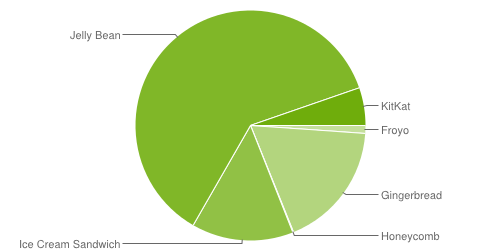
\includegraphics[width=.85\textwidth]{figuras/chart.png}
  \caption{Distribuição das versões do Android}
  \label{fig:d}
\end{figure}

\newpage
Esse material irá cobrir alguns tópicos no desenvolvimento de aplicativos para android, tais como:
\bi
\item
Configuracão do ambiente de desenvolvimento: Como configurar o ambiente para começar a desenvolver aplicativos, os primeiros passos para criar seu primeiro aplicativo de maneira simples;
\item
Elementos da interface: Como projetar seu aplicativo para usar as principais interfaces. Listas, Listas compostas, Grades, Abas, Menus são as interfaces mais usadas nos diversos aplicativos no mercado; e
\item
Elementos de hardware: Como projetar seu aplicativo para usar as APIs de hardware: Bluetooth, GPS, SMS, Chamadas.
\ei

 Para esse material, algumas convenções serão seguidas: 
 \bi
 \item
Os códigos estarão sempre com a sintaxe colorida para facilitar a leitura;
\item
URLs das referências estarão nas notas de rodapé; e
\item
 Dicas estarão envoltas por uma caixa para facilitar a visualização
\ei

% http://tug.ctan.org/tex-archive/macros/latex/contrib/minted/
% http://pygments.org/

\cha{configambiente}{Configuração do Ambiente}
A instalação e configuração do ambiente de desenvolvimento para Android é simples, o Google fornece um pacote chamado ADT \emph{(Android Development Tools)} que contém o ambiente Eclipse com o \emph{plugin} do Android, algumas ferramentas para instalação dos aplicativos nos \emph{smartphones}, o gerenciador do SDK e as imagens para o emulador do Android. Essas ferramentas são suficientes para o desenvolvimento na plataforma.
O pacote ADT pode ser encontrado em: \href{http://developer.android.com/sdk/}{Android SDK}\footnote{\href{http://developer.android.com/sdk/}{http://developer.android.com/sdk/}}. 

Basta fazer o download do pacote e extrair que tudo já está pré-configurado para iniciar o desenvolvimento, portanto não há muito o que configurar.

Caso opte por utilizar uma instalação já existente do ambiente Eclipse, você pode instalar o plugin do Android automaticamente através da ferramenta de instalação de plugins do ambiente. Após a instalação será necessário abrir o \emph{SDK Manager} e instalar:
\begin{itemize}[noitemsep, nolistsep]
\item \emph{Android SDK Tools};
\item \emph{Android SDK Platform-Tools}; e
\item Para cada API que você irá utilizar, instalar o \emph{SDK Platform} e opcionalmente o \emph{Documentation for Android SDK} e o \emph{Samples for SDK}.
\end{itemize}

\cha{intro-android}{Linguagem do Android}
\section{Linguagem}
A linguagem usada para programar na plataforma Android é Java. Então antes de engajar no aprendizado Android é altamente recomendável estudar material Java e principalmente o paradigma de orientação a objetos.

O Android tem algumas particulariedades na organização e configuração que é feita através de arquivos XML específicos do Android. Alguns arquivos XML servem para configurar o aplicativo, layout de cada tela e outros dão suporte a strings para facilitar o suporte a múltiplos idiomas.
Felizmente o conjunto Eclipse com ADT já cuida disso automaticamente e possui uma serie de facilidades alcançadas por meio de interfaces gráficas para os programadores. Por esse motivo, para qualquer iniciante nessa área e recomendável a utilizacão do ambiente Eclipse.

A criação de layouts dos aplicativos pode ser feita inteiramente através da interface gráfica disponível no ambiente, no estilo \textit{drag and drop}. 

\section{Entendendo a estrutura de uma aplicação Android}

Uma aplicação Android consiste de uma ou mais \emph{activities}. Uma \emph{activity} é uma tela com \emph{views} que interagem com o usuário. Como o Android segue o padrão MVC \emph{(Model-View-Control)} as \emph{activities} são os \emph{controllers} e as \emph{views}, \emph{views}. As \emph{activities} são classes do Java, o \emph{layout} e outros recursos são definidos em arquivos XML.

Dentre os diversos arquivos XML existentes na configuração de um aplicativo Android o mais importante é o \texttt{{AndroidManifest.xml}}
\footnote{Documentação do \texttt{AndroidManifest}: \href{The AndroidManifest.xml File}{http://developer.android.com/guide/topics/manifest/manifest-intro.html}}
 pois é nele que se exprimem as configurações gerais do aplicativo. Nesse texto não iremos adentrar muito nos detalhes das configurações, mas apenas deixar claro que é nesse arquivo que se colocam as versões do Android que seu aplicativo será compatível com, as permissões para usar os recursos do aparelho como Internet, GPS, Bluetooth, etc. 
 
 A pasta \texttt{src/} contém o pacote com as classes do seu aplicativo isto é, o código fonte do seu aplicativo. Tanto \emph{activites} como classes de suporte devem estar dentro do pacote.

Dentro da pasta \texttt{res/} de recursos, encontram-se outros arquivos, referentes à disposição do layout, valores de strings e imagens que sua aplicação irá utilizar. A pasta \texttt{layout/} junto com as pastas \texttt{drawable-*/} servem para dispor o layout. Cada \textit{drawable} comporta imagens para um tamanho diferente de tela, enquanto que a pasta de \textit{layout} contém a dispoção geral do layout. São nesses arquivos que se colocam os itens \emph{(views)} que irão nas telas, como botões, caixas de texto, caixas de seleção, etc.

Na pasta \texttt{values/} o mais importante é o arquivo \texttt{strings.xml} que contém os valores das strings do aplicativo. Sempre que você quiser referenciar alguma string, a mesma deverá estar expressa nesse arquivo. Fica fácil dessa forma fazer o aplicativo suportar múltiplos idiomas, pois basta traduzir esse único arquivo para alterar todos os textos do aplicativo.

A pasta \texttt{menu/} contém os \emph{layouts} do menus do aplicativo, esses são aqueles que podem ser acessados através da \emph{Action Bar}\footnote{\emph{ActionBar}: \href{http://developer.android.com/design/patterns/actionbar.html}{http://developer.android.com/design/patterns/actionbar.html}} ou através dos botões físicos do aparelho.

\newpage
\textbf{Resumindo:}
\begin{itemize}[noitemsep, nolistsep]
\item \texttt{AndroidManifest.xml}: Configurações gerais do aplicativo;
\item \texttt{src/}: Classes do aplicativo; e
\item \texttt{res/}: Recursos do aplicativo tais que:
	\begin{itemize}[nolistsep, noitemsep]
		\item \texttt{strings/}: Todos os textos da sua aplicação, suporte a múltiplos idiomas;
		\item \texttt{layout/}: Todos os \emph{layouts} de suas telas \emph{(activites)};
		\item \texttt{drawable/}: Todas as imagens, separados por tamanho de tela; e
		\item \texttt{menu/}: \emph{layout} dos menus do aplicativo.
	\end{itemize}
\end{itemize}


%% FIRST APP %%
\cha{primeiro-aplicativo}{Criando seu primeiro aplicativo}
Para exemplificar a criação de um aplicativo, seguiremos o exemplo dado pelo próprio manual do Google sobre o Android 
(Ver original\footnote{Original em: \href{http://developer.android.com/training/basics/firstapp/creating-project.html}{http://developer.android.com/training/basics/firstapp/creating-project.html}}). 
Trata-se de aplicativo simples do tipo \emph{''Hello World''}.

Iniciaremos criando um novo projeto no Eclipse acessando o menu: \emph{File -> New -> Android Application Project}.

Na janela que apareceu você deve colocar o nome do aplicativo, do projeto e do pacote. O nome do pacote deve seguir a convenção do Java\footnote{Convenção sobre nome dos pacotes: \href{http://docs.oracle.com/javase/tutorial/java/package/namingpkgs.html}{http://docs.oracle.com/javase/tutorial/java/package/namingpkgs.html}}.
\begin{itemize}[noitemsep]
	\item \textit{Minimum Required SDK:} É a versão mínima do sistema operacional Android que sua aplicação irá suportar, o mais comum é a versão 8 do SDK que se refere ao Android 2.2. Alguns tipos de layouts mais complexos não são suportados em versões mais antigas;
	\item \textit{Target SDK:} É a versão principal do Android para qual seu aplicativo está sendo desenvolvido;
	\item \textit{Compile With:} Versão do Android com qual seu aplicativo será compilado; e
	\item \textit{Theme:} Cores do layout.
\end{itemize}


\begin{figure}[H]
  \centering
  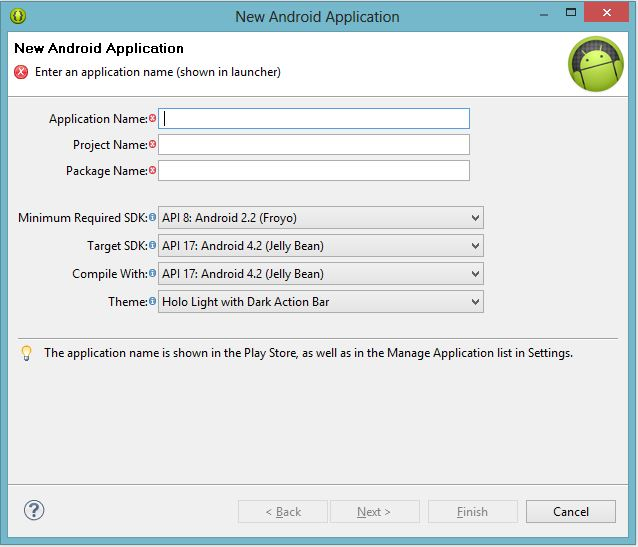
\includegraphics[width=.8\textwidth]{figuras/1-criando-app.jpg}
  \caption{Primeira janela de criação de novo aplicativo}
  \label{fig:d}
  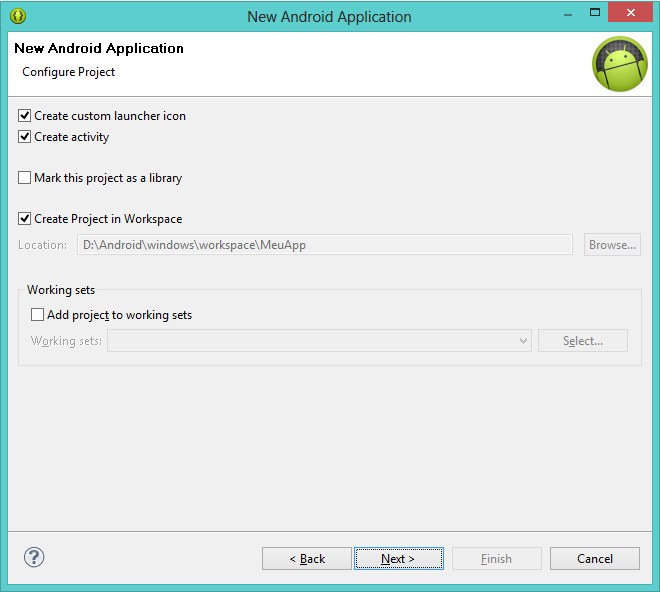
\includegraphics[width=.8\textwidth]{figuras/2-criando-app-2.png}
  \caption{Segunda janela de criação de novo aplicativo}
  \label{fig:c}
\end{figure}
\newpage
\begin{figure}[H]
  \centering
  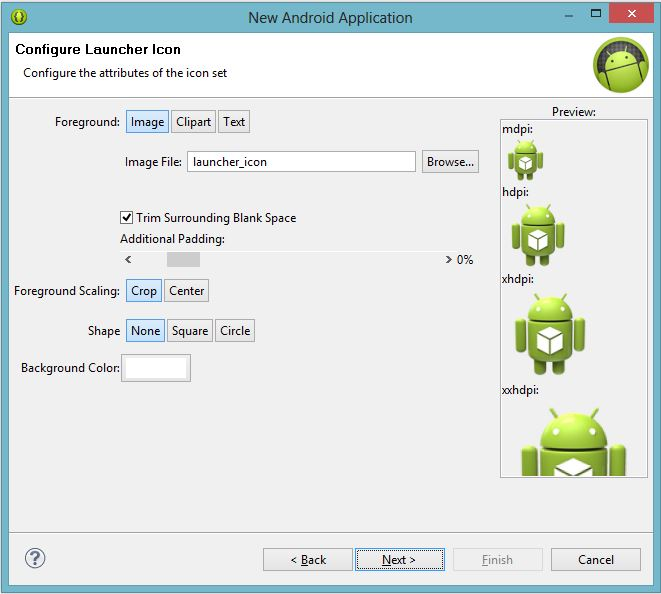
\includegraphics[width=.8\textwidth]{figuras/2-criando-app.jpg}
  \caption{Terceira janela de criação de novo aplicativo}
  \label{fig:c}
   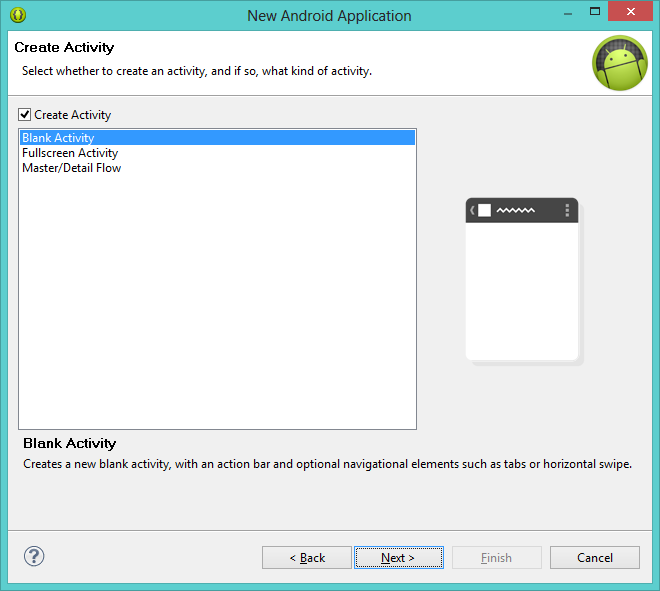
\includegraphics[width=.8\textwidth]{figuras/2-criando-app-4.png}
  \caption{Quarta janela de criação de novo aplicativo}
  \label{fig:c}
 \end{figure}
 \newpage
\begin{figure}[H]
  \centering
   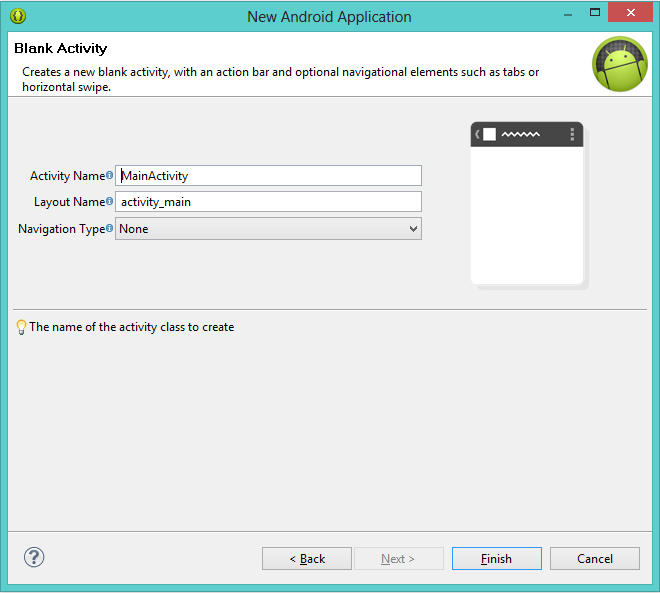
\includegraphics[width=.8\textwidth]{figuras/2-criando-app-5.png}
  \caption{Quinta janela de criação de novo aplicativo}
  \label{fig:c}
\end{figure}
\newpage
Observe na Figura 4.1 a janela de criação de uma nova aplicação Android. Em \emph{Application Name} você deve colocar o nome do aplicativo, em \emph{Project Name}, o nome do projeto e em \emph{Package Name} o nome do pacote. Para esse exemplo utilizaremos como \emph{Minimum Required SDK} a versão API 8, já que nesse exemplo não usaremos nenhum layout que não é suportado em versões mais antigas. Em \emph{Target SDK} e \emph{Compile With} optaremos pela versão mais nova, a API 17. Por final o \emph{Theme} eu optei pelo \emph{Holo Light with Dark Action Bar} que é um tema com fundo branco e barra superior preta, um dos padrões do Android.

\begin{framed}
\textbf{Dica:} Para obter o máximo de compatibilidade sempre procure utilizar \emph{layouts} compatíveis com versões antigas, observe na figura 1.1 que versões antigas ainda tem uma fatia considerável do mercado.
\end{framed}

A figura 4.2 mostra a segunda janela da configuração inicial do seu aplicativo. Você pode escolher um ícone personalizado se marcar a caixa \emph{Create custom launcher icon} o que te levará para a janela da figura 4.3. Se marcar \emph{Create Activity}  o assistente de criação te levará para a janela da figura 4.4 onde poderá escolher qual \emph{activity} vai ser criada para seu aplicativo. Em todos os exemplos escolheremos a opção \emph{Blank Activity}. Como nosso projeto não e uma biblioteca não marcaremos \emph{Mark this project as a library}. Se marcar \emph{Create Project in Workspace} o assistente irá salvar o projeto na pasta que foi configurada para o \emph{Workspace}, caso contrário ele irá pedir para escolher outro caminho. Como não trabalharemos com \emph{Working Sets} do Eclipse, a opção \emph{Add project to working sets} permanece desmarcada. 

Finalmente a figura 4.5 mostra a janela para nomear a \emph{activity} inicial, nesse exemplo mantive \emph{MainActivity}. O nome do \emph{layout} dessa \emph{activity} mantive como \emph{activity\_main} que é o padrão. Na caixa \emph{Navigation Type} existem algumas opções de \emph{layout} pré-definidas pelo Android. São elas:
\begin{itemize}[noitemsep, nolistsep]
\item
	\emph{None:} O \emph{layout} vem apenas com uma \emph{Action Bar}\footnote{Documentação da \emph{ActionBar}: \href{http://developer.android.com/guide/topics/ui/actionbar.html}{http://developer.android.com/guide/topics/ui/actionbar.html}}
\item
	\emph{Fixed Tabs + Swipe:} O \emph{layout} vem com algumas abas e com gesto de arrastar entre as abas \emph{(activities)} pré-programados.
	\footnote{\emph{Tabs:} \href{http://developer.android.com/design/building-blocks/tabs.html}{http://developer.android.com/design/building-blocks/tabs.html}}
\item
	\emph{Scrollable Tabs + Swipe:} O \emph{layout} vem com algumas abas e com gesto de arrastar entre as abas pré-programados, porém nesse o estilo das abas é diferente, em vez de abas fixas, são abas que movem para dar espaço a outras. 
\item
	\emph{Dropdown}: O \emph{layout} vem com a troca de \emph{activites} através de um menu na \emph{Action Bar}.  
\end{itemize}


\begin{singlespace}
\begin{listing}[H]
\inputminted[linenos=true,fontsize=\small,frame=lines, framesep=2mm, tabsize=2,numbersep=5pt]{xml}{src/firstapp/sdk-manifest.xml}
\label{AndroidManifest.sdk}
\caption{Exemplo de configuração de versão do SDK no \texttt{\textcolor{mygreen}{AndroidManifest.xml}} }
\end{listing}

Primeiro vamos criar um layout para o aplicativo usando a interface gráfica do Eclipse, primeiro abra o arquivo \texttt{\textcolor{mygreen}{res/layout/activity\_main.xml}} , segundo o AndroidManifest, é essa \emph{activity} que será aberta quando o aplicativo for iniciado, configurado através do \textit{intent-filter}. Cada \emph{activity} é uma tela do aplicativo e é responsáve primariamente por mostrar as informações, o Android segue o modelo \emph{MVC} \textit{(Model-View-Control)}, e as \emph{activity} são as \textit{Views} do aplicativo.
\begin{listing}
\begin{minted}[mathescape,
               linenos,
               numbersep=5pt,
               tabsize=2,
               frame=lines,
               framesep=2mm]{xml}
<intent-filter>
	<action android:name="android.intent.action.MAIN" />
	<category android:name="android.intent.category.LAUNCHER"/>
</intent-filter>
\end{minted}
\caption{Configuração dos \textit{intent-filters} no \texttt{\textcolor{mygreen}{AndroidManifest.xml}} }
\end{listing}

Não entraremos em detalhes sobre os \textit{intent-filters} agora. Selecione o ''Hello world'' e delete ele da sua \emph{activity}

\begin{figure}[H]
  \centering
  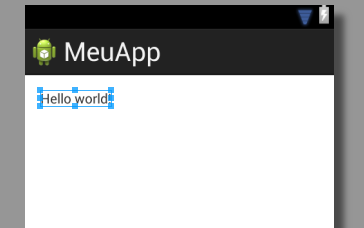
\includegraphics{figuras/3-criando-app.png}
  \caption{Selecionando o Hello world}
  \label{fig:b}
\end{figure}

Agora arraste um \textit{Text Field -> Plain Text} e um \textit{Form Widgets -> Button} para sua \emph{activity} 

\begin{figure}[H]
  \centering
  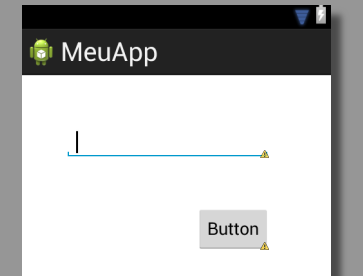
\includegraphics{figuras/4-criando-app.png}
  \caption{\emph{activity} com os elementos colocados na tela}
  \label{fig:a}
\end{figure}

Ao clicar duas vezes no elemento no modo visual, você sera levado ao correspondente marcador desse elemento no XML correspondente da \emph{activity}. Clique duas vezes na caixa de texto.

\begin{listing}
\inputminted[linenos=true,fontsize=\small,frame=lines, framesep=2mm, tabsize=2,numbersep=5pt]{xml}{src/firstapp/1.xml}
\caption{Código da caixa de texto}
\end{listing}

Primeiro, modifique a \textit{id} para um mais intuitivo, por exemplo você pode chama-lo de \textit{caixaTextoNome}. Todo \textit{id} deve ser precedido de \texttt{@+id/} como definido pelo Android. Os outros atributos são para definir o tamanho, alinhamento e margem, todos relativos ao elemento pai desse elemento que no caso é o próprio layout. Depois adicione uma \textit{hint} para essa caixa de texto, uma \textit{hint} é algo que vai estar escrito na caixa de texto quando ela estiver vazia, indicando que tipo de texto você pretende que seja escrito nessa caixa de texto, essa \textit{hint} é uma referência a \texttt{string} chamada \texttt{nome} que está definida no arquivo \texttt{\textcolor{mygreen}{res/values/strings.xml}}.	 No código acima a \textit{hint} já foi colocada na linha 10.

Depois modifique o código do botão, trocando o \textit{id} e as referências ao \textit{id} da caixa de texto, também edite o \texttt{android:text} para fazer uma referência a uma string no arquivo de strings. Por último adicione um atributo \texttt{android:onClick} que é o método que será executado quando o botão for pressionado.

\begin{listing}[H]
\inputminted[linenos=true,fontsize=\small,frame=lines, framesep=2mm, tabsize=2,numbersep=5pt]{xml}{src/firstapp/2.xml}
\caption{Código do botão}
\end{listing}

Adicione as strings ao arquivo de strings, essas strings podem ser referenciadas a qualquer momento tanto na construção do layout como na codificação do aplicativo.

\begin{listing}
\inputminted[linenos=true,fontsize=\small,frame=lines, framesep=2mm, tabsize=2,numbersep=5pt]{xml}{src/firstapp/3.xml}
\caption{Arquivo de strings com as duas strings adicionadas}
\end{listing}

Agora abra a classe \texttt{MainActivity} localizada na pasta \texttt{\textcolor{mygreen}{src/}} do seu projeto e adicione um novo método

\begin{listing}
\inputminted[linenos=true,fontsize=\small,frame=lines, framesep=2mm, tabsize=2,numbersep=5pt]{java}{src/firstapp/4.java}
\caption{Adicionando método à classe MainActivity}
\end{listing}

\bi
\item{Isso vai requer você importe a classe View, você pode apertar \texttt{Ctrl+Shit+O} no Eclipse para importar classes que estejam faltando}
\ei

\begin{listing}
\inputminted[linenos=true,fontsize=\small,frame=lines, framesep=2mm, tabsize=2,numbersep=5pt]{java}{src/firstapp/4-2.java}
\caption{Exemplo de import de classe Android}
\end{listing}


Primeiro, crie um novo \texttt{Intent}\footnote{Documentação Intent: \href{http://developer.android.com/reference/android/content/Intent.html}{http://developer.android.com/reference/android/content/Intent.html}}, um \texttt{Intent} é um objeto que providencia uma ligação entre dois componentes separados (tais como duas \textit{activities}). O \texttt{Intent} representa uma ''intenção do aplicativo de fazer algo'', eles podem ser usados para uma variedade de tarefas, mas são principalmente usados para iniciar uma nova \emph{activity}.

\begin{listing}[H]
\inputminted[linenos=true,fontsize=\small,frame=lines, framesep=2mm, tabsize=2,numbersep=5pt]{java}{src/firstapp/5.java}
\caption{Adicionando uma \texttt{Intent}}
\end{listing}

Agora você precisa obter o texto que está escrito na caixa para fazer algo com ele, no caso iremos enviar para outra \emph{activity} que irá mostrar esse texto.

\begin{listing}[H]
\inputminted[linenos=true,fontsize=\small,frame=lines, framesep=2mm, tabsize=2,numbersep=5pt]{java}{src/firstapp/6.java}
\caption{Obtendo o conteúdo da caixa de texto e enviando para outra \emph{activity}}
\end{listing}

O código na linha 3 está obtendo a referência a caixa de texto usando o método \texttt{findViewById()} e o argumento passado é o \textit{id} da caixa de texto, observe que você chama com \texttt{R.id.caixaTextoNome} isso é feito dessa forma porque o android compila automaticamente uma classe R (R de \textit{Resources}) que contém as \textit{id's} e \textit{strings} criadas nos arquivos XML.
Em seguida usando o método \texttt{getText()} da caixa de texto, obtem-se a string que foi escrita lá.

Por fim, essa string é colocada no \texttt{Intent} com o método \texttt{putExtra()}, uma \texttt{Intent} pode carregar consigo uma coleção de vários tipos de dados como pares chave-valor chamados \textit{extras}, esse método toma a chave como primeiro parâmetro e o valor no segundo parâmetro.
Para que a próxima \emph{activity} consiga coletar esse valor, você deve definir uma chave para seu \textit{extra} usando uma constante pública. Para isso adicione a definição de \texttt{EXTRA\_MESSAGE} no topo da sua classe \texttt{MainActivity}.

\begin{listing}[H]
\inputminted[linenos=true,fontsize=\small,frame=lines, framesep=2mm, tabsize=2,numbersep=5pt]{java}{src/firstapp/7.java}
\caption{Constante como chave para um extra}
\end{listing}

Agora você deve criar uma nova \emph{activity}, para isso vá em \textit{File -> New -> Other -> Android Activity} e selecione \textit{Blank Activity}. Preencha a próxima janela dessa maneira, depois clique \textit{Finish}. 

\begin{figure}[H]
  \centering
  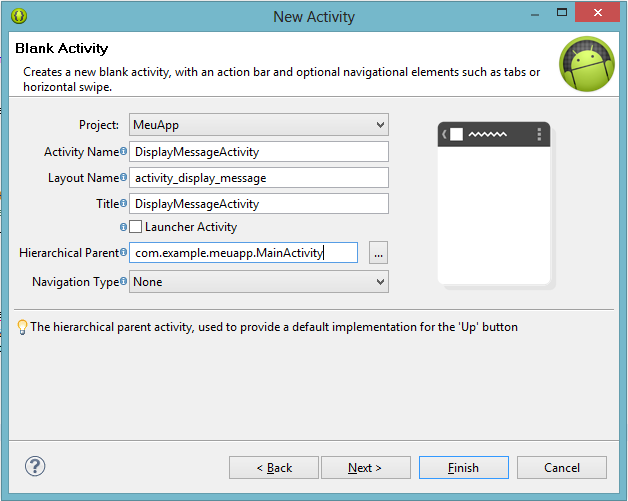
\includegraphics[width=1\textwidth]{figuras/5-criando-app.png}
  \caption{Criando uma nova \emph{activity}}
  \label{fig:e}
\end{figure}

A classe já vem com alguns métodos implementados, alguns não serão necessários para esse aplicativo, mas mantenha eles na classe. Todas as classes que são subclasses de \emph{activity} precisam implementar o método \texttt{onCreate()}\footnote{\href{http://developer.android.com/reference/android/app/Activity.html\#onCreate(android.os.Bundle)}{http://developer.android.com/reference/android/app/Activity.html\#onCreate(android.os.Bundle)}}.

Geralmente você precisaria adicionar uma nova string com o nome da classe no XML, e adicionar a \emph{activity} no \texttt{\textcolor{mygreen}{AndroidManifest.xml}} porém como estamos trabalhando com o Eclipse, você não precisa se preocupar que ele faz isso sozinho.

Agora, precisamos extrair os dados enviados a essa \emph{activity} através do \texttt{intent}, você pode pegar o \texttt{intent} que começou a \emph{activity} chamando o método \texttt{getIntent()}\footnote{\href{http://developer.android.com/reference/android/app/Activity.html\#getIntent()}{http://developer.android.com/reference/android/app/Activity.html\#getIntent()}}.

\begin{listing}[H]
\inputminted[linenos=true,fontsize=\small,frame=lines, framesep=2mm, tabsize=2,numbersep=5pt]{java}{src/firstapp/8.java}
\caption{Obtendo extras passados através do \texttt{Intent}}
\end{listing}

Agora para mostrar a mensagem na tela, você precisa criar um \texttt{TextView}\footnote{\href{http://developer.android.com/reference/android/widget/TextView.html}{http://developer.android.com/reference/android/widget/TextView.html}}

\begin{listing}[H]
\inputminted[linenos=true,fontsize=\small,frame=lines, framesep=2mm, tabsize=2,numbersep=5pt]{java}{src/firstapp/9.java}
\caption{Método \texttt{onCreate()} recebendo um \texttt{Intent} e mostrando a mensagem}
\end{listing}

Agora que o aplicativo está pronto, é necessário testar, caso tenha um smartphone Android você pode conectá-lo no seu computador e rodar diretamente, senão você deverá rodar em um emulador.


Para rodar diretamente no smartphone:
\be
\item Conecte seu smartphone no computador através do cabo USB. Se estiver desenvolvendo no Windows será preciso instalar os drivers USB do seu dispositivo. Se precisar de ajuda para instalar os drivers acesse: \href{http://developer.android.com/tools/extras/oem-usb.html}{OEM USB}\footnote{\href{http://developer.android.com/tools/extras/oem-usb.html}{http://developer.android.com/tools/extras/oem-usb.html}}
\item Ative o modo \emph{USB Debugging} no dispositivo
	\bi
	\item Para Android 3.2 ou mais antigos, a opção deve estar em \textit{Configurações -> Aplicativos	 -> Desenvolvimento}
	\item Para Android 4.0 e 4.1, a opção está em \textit{Configurações -> Opções do desenvolvedor}
	\item Para Andoird 4.2 e mais novos, a opção está escondida por padrão, para mostrar a opção você deve entrar em \textit{Sobre o telefone} e clicar em \textit{Número da versão} 7 vezes, ao retornar para tela anterior deverá aparecer \textit{Opções do desenvolvedor}
	\ei
\ee

\newpage 
Para rodar no emulador:
\be
\item Abra o \textit{SDK Manager} através do Eclipse em: \textit{Window -> Android SDK Manager}
\item Verifique se, para Android 4.2.2 (API 17) ou outro desejado os seguintes pacotes estejam instalados
	\bi
	\item \textit{SDK Platform}
	\item \textit{ARM EABI v7a System Image} ou
	\item \textit{Intel x86 Atom System Image}
	\ei
\item Verifique também se em \textit{Tools}, os pacotes \textit{Android SDK Tools} e \textit{Android SDK Platform-tools} estão instalado
\item Agora é necessário criar um AVD (Android Virtual Device\footnote{\href{http://developer.android.com/tools/devices/index.html}{http://developer.android.com/tools/devices/index.html}}), no Eclipse vá em \textit{Window -> Android Virtual Device Manager} 
\item No AVD Manager clique em \emph{New}
\item Complete as informações do AVD, dê um nome, plataforma, espaço de armazenamento, quantidade de memória RAM
\item Clique \emph{Create AVD}
\item Selecione o novo AVD no \textit{Android Virtual Device Manager} e clique \emph{Start}
\item Quando o emulador terminar de carregar, destrave a tela do emulador
\ee

Agora para rodar o aplicativo basta clicar em \emph{Run} na barra de tarefas do Eclipse e selecionar \textit{Android Application} na janela \emph{Run as}. O Eclipse irá instalar o APK e abrir o aplicativo automaticamente.

\begin{figure}[H]
  \centering
  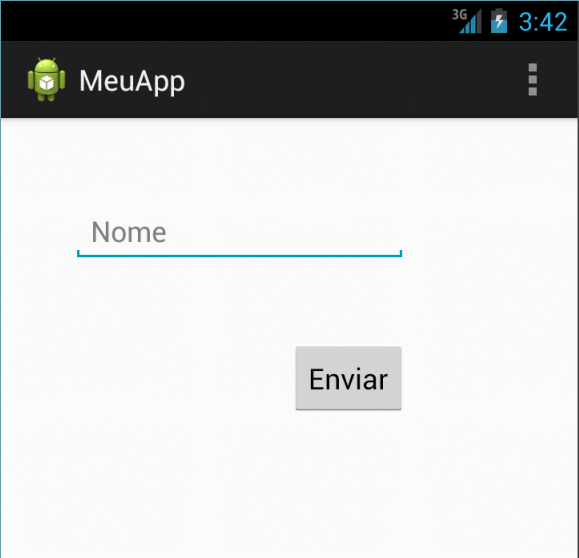
\includegraphics[width=.4\textwidth]{figuras/6-criando-app.png}
  \caption{Primeira tela do primeiro aplicativo}
  \label{fig:f}
  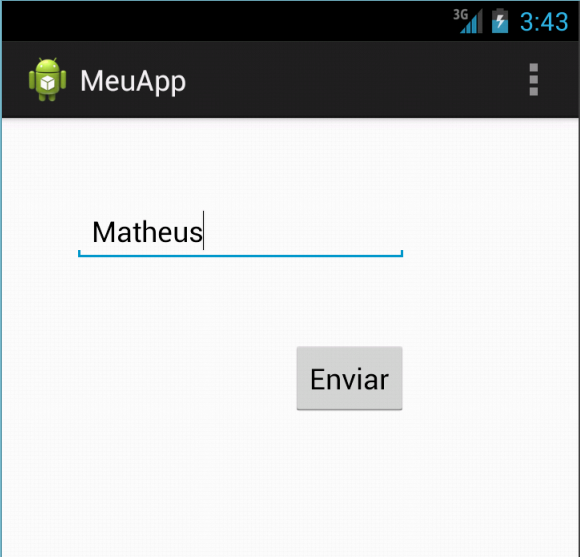
\includegraphics[width=.4\textwidth]{figuras/7-criando-app.png}
  \caption{Primeira tela após escrever texto na caixa de texto}
  \label{fig:g}
\end{figure}
\begin{figure}[H]
  \centering
  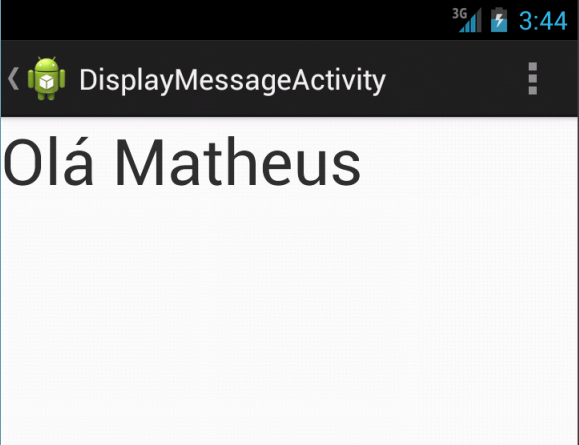
\includegraphics[width=.4\textwidth]{figuras/8-criando-app.png}
  \caption{Segunda tela mostrando a mensagem enviada}
  \label{fig:h}
\end{figure}

%%%%%%% DESIGN %%%%%%%%%%
\cha{design}{Design}

%%% ACTIVITY %%%
\section{Activity}
Enquanto um usuário navega pelas variadas telas de um aplicativo, sai dele e volta depois, as instâncias de uma \emph{activity} transitam dentre diferentes estados em seu ciclo de vida. Quando um aplicativo é iniciado, uma \emph{activity} inicial é criada o sistema invoca métodos específicos que correspondem a criação dessa \emph{activity}. Durante todo o ciclo de vida vários métodos são chamados, e todos eles correspondem a diferentes estágios desse ciclo de vida. 

Observe na imagem abaixo os métodos correspondentes a cada estado da vida de uma \emph{activity}, quando ela é criada o método \texttt{onCreate()} é o responsável pela configuracão inicial. O sistema ao criar uma nova instância de uma \emph{activity}, cada método muda o estado da \emph{activity} um degrau pra cima na pirâmide. 

% COLOCAR FONTE: http://developer.android.com/training/basics/activity-lifecycle/starting.html %
\begin{figure}[H]
  \centering
  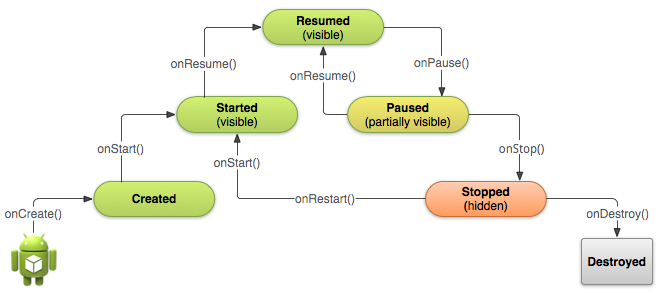
\includegraphics[width=1\textwidth]{figuras/design/basic-lifecycle.png}
  \caption{Ciclo de vida de uma \emph{activity} }
  \label{fig:e}
\end{figure}

Assim que o usuário começa a sair da \emph{activity}, o sistema invoca outros métodos que movem o estado para níveis mais baixos da pirâmide para começar a desmontar a \emph{activity}. Em alguns casos a \emph{activity} irá apenas ir até certo ponto e esperar (por exemplo quando o usuário troca para outro aplicativo) tal que ela possa voltar de onde parou caso o usuário volte. 

 Não são todos métodos que precisam ser implementados pois isso irá depender da complexidade do seu aplicativo. É importante salientar porém que, implementar esses métodos irá garantir que seu aplicativo se comporte de maneira correta, por exemplo você deve garantir que:
 \bi
 \item Seu aplicativo não falhe quando o usuário receber uma chamada telefônica ou quando o usuário troca de aplicativo;
 \item Seu aplicativo não consuma recursos do sistema enquanto não estiver sendo usado;
 \item Seu aplicativo não perca o progresso do usuário; e
 \item Seu aplicativo não falhe ou perca o progresso do usuário quando a tela rotaciona entre retrato e paisagem.
\ei

Apenas três dentre os estados são estáticos, isto é, a \emph{activity} pode ficar nesse estado por um longo período de tempo:


Retomado \emph{(Resumed)}
	
\hspace*{5mm} Nesse estado a \emph{activity} está em primeiro plano e o usuário pode interagir com ela.
	
Pausado \emph{(Paused)}
	
\hspace*{5mm} Nesse estado a \emph{activity} está parcialmente obscurecida por outra \emph{activity} - a outra \emph{activity} que está em primeiro plano é semi-transparente ou não ocupa todo espaço da tela. A \emph{activity} quando pausada não consegur interagir com o usuário e não executa nenhum código.
	
Parado \emph{(Stopped)}
	
\hspace*{5mm} Nesse estado a \emph{activity} está completamente oculto e não está visível para o usuário, está em plano de fundo. Quando está parada, uma instância de uma \emph{activity} e toda informação de seu estado tais como variáveis são mantidos, porém a \emph{activity} não executa nenhum código.
	
\section{Especifique a \emph{activity} que inicia seu aplicativo}

Quando um usuário abre um aplicativo, o sistema chama o método \texttt{onCreate()} da \emph{activity} que foi declarada como sendo a iniciadora do aplicativo. Você pode definir qual \emph{activity} que vai iniciar seu aplicativo no arquivo \texttt{AndroidManifest.xml} que está no diretório raíz do seu projeto.

 A \emph{activity} que inicia seu aplicativo deve ser declarada no manifesto com um \texttt{<intent-filter>}\footnote{Documentação \texttt{<intent-filter>}: \href{http://developer.android.com/guide/topics/manifest/intent-filter-element.html}{http://developer.android.com/guide/topics/manifest/intent-filter-element.html}} que inclui a \texttt{<action>} MAIN e a \texttt{<category>} LAUNCHER. Por exemplo:
 
\begin{listing}[H]
\inputminted[linenos=true,fontsize=\small,frame=lines, framesep=2mm, tabsize=2,numbersep=5pt]{xml}{src/design/launcher-manifest.xml}
\caption{Exemplo de \emph{Launcher activity}}
\end{listing}

%dica
\begin{framed}
\textbf{Dica:} Quando você cria um projeto Android no Eclipse, por padrão é incluida uma classe \emph{activity} que está declarada no manifesto com esse filtro.
\end{framed}


%%% LIST VIEW %%%%
\section{Listas \texttt{(ListView)}}\footnote{Documentação \texttt{ListView}:\href{http://developer.android.com/reference/android/widget/ListView.html}{http://developer.android.com/reference/android/widget/ListView.html}}
Listas são uma das formas mais simples e mais poderosas de se mostrar informações ao usuário de forma simples e objetiva, a \texttt{ListView} é altamente customizável através de adaptadores.

\begin{figure}[H]
  \centering
  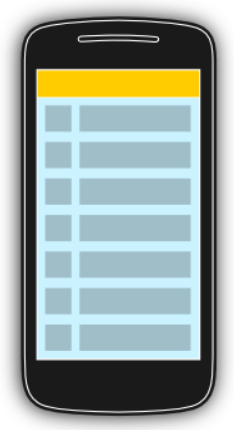
\includegraphics[width=.15\textwidth]{figuras/design/listview-scheme.png}
  \caption{Esquema de uma lista}
  \label{fig:e}
\end{figure}

Um item individual da lista pode ser selecionado, essa seleção pode acionar uma outra tela com detalhes do item.


\begin{figure}[H]
  \centering
  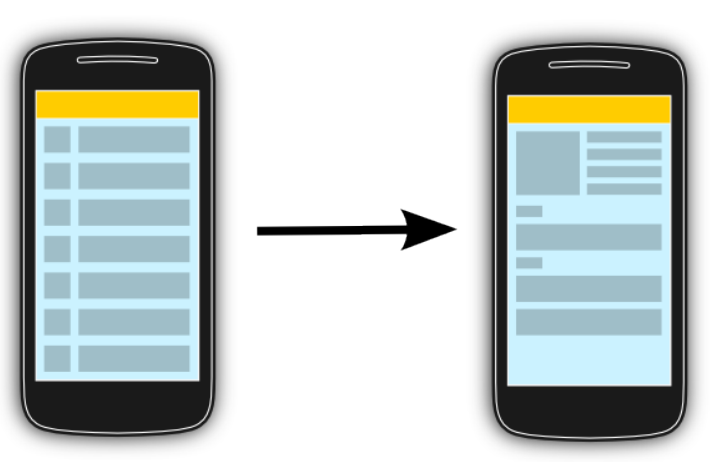
\includegraphics[width=.35\textwidth]{figuras/design/listview-scheme2.png}
  \caption{Detalhes de um elemento da lista}
  \label{fig:e}
\end{figure}

\newpage

A construção é simples, você pode começar mudando o layout de \texttt{RelativeLayout} para \texttt{LinearLayout}, a diferença entre eles é que o \texttt{RelativeLayout} do exemplo passado permite você posicionar elementos uns relativos aos outros enquanto que o \texttt{LinearLayout} segue uma estrutura, vertical ou horizontal. Ambas podem ser aninhadas uma dentro de outra.

\begin{listing}[H]
\inputminted[linenos=true,fontsize=\small,frame=lines, framesep=2mm, tabsize=2,numbersep=5pt]{xml}{src/design/layout_linear.xml}
\caption{Layout \textit{Linear} no \texttt{activity\_main.xml}}
\end{listing}

Agora, você pode arrastar um \texttt{ListView} para o layout ou criar um manualmente com o seguinte código XML

\begin{listing}[H]
\inputminted[linenos=true,fontsize=\small,frame=lines, framesep=2mm, tabsize=2,numbersep=5pt]{xml}{src/design/listview.xml}
\caption{Código XML de um \texttt{ListView}}
\end{listing}

Agora para popular a lista, você precisa criar um \texttt{string-array} no arquivo \texttt{\textcolor{mygreen}{strings.xml}} com os elementos que deseja colocar na lista.

\begin{listing}[H]
\inputminted[linenos=true,fontsize=\small,frame=lines, framesep=2mm, tabsize=2,numbersep=5pt]{xml}{src/design/string-array.xml}
\caption{\texttt{string-array} populada com elementos}
\end{listing}

E por final, escrever o código que irá preencher a lista com as \textit{strings} desse \textit{array}.

\begin{listing}[H]
\inputminted[linenos=true,fontsize=\small,frame=lines, framesep=2mm, tabsize=2,numbersep=5pt]{java}{src/design/listactivity.java}
\caption{Código de uma \emph{activity} com lista clicável}
\end{listing}

Adaptadores são usados para prover dados para o \texttt{ListView}, ele define como cada linha será mostrada. Um adaptador extende a classe \texttt{BaseAdapter}, o Android provê alguns adaptadores padrões, no caso estamos usando o \texttt{ArrayAdapter} que é para manusear dados em \textit{arrays}.

Dentro da interface \texttt{OnItemClickListener} você pode configurar a ação de clicar em um dos itens da lista, nesse exemplo é criado um \texttt{Toast} que mostra uma mensagem com o texto do item na lista porém, qualquer ação pode ser executada incluindo abrir uma nova \emph{activity} que esteja relacionada a esse item.

Você pode também herdar da classe \texttt{ListActivity} para uma forma mais simples de manusear \texttt{ListViews}. Você não precisa atribuir um layout a \texttt{ListActivity} contém uma \texttt{ListView} padrão. Caso voce precise colocar mais \texttt{Views} em seu layout, você \emph{deve} colocar a \texttt{ListView} em seu layout com o id \texttt{''@android:id/list''}.

\begin{figure}[H]
  \centering
  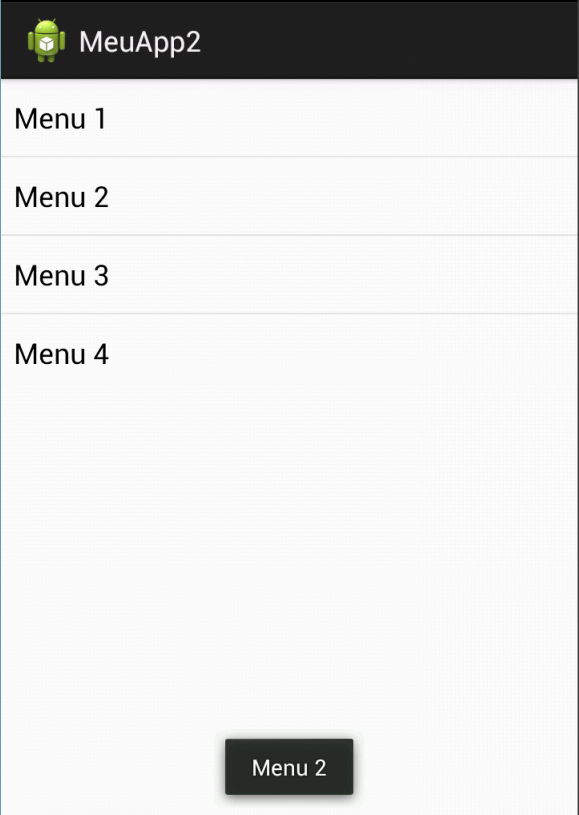
\includegraphics[width=.7\textwidth]{figuras/design/lista.png}
  \caption{Lista simples}
  \label{fig:e}
\end{figure}

Obs.: O \texttt{Toast} é esse pequeno retângulo preto com uma mensagem, ele aparece e desaparece rapidamente apenas para mostrar uma mensagem ao usuário.

%%% LIST ADAPTER %%%
\section{Listas Compostas}
É possível compor um item da lista colocando mais elementos no mesmo além de um texto. Para isso você precisa criar um novo arquivo XML que irá definir a customização de cada linha de uma \texttt{ListView}, defina um arquivo chamado \texttt{\textcolor{mygreen}{item.xml}}.

\newpage

\begin{listing}[H]
\inputminted[linenos=true,fontsize=\small,frame=lines, framesep=2mm, tabsize=2,numbersep=5pt]{xml}{src/design/item.xml}
\caption{Código do arquivo \texttt{\textcolor{mygreen}{item.xml}}}
\end{listing}	

Agora você precisa usar um adaptador para mostrar esse layout customizado em cada linha da lista, uma maneira fácil é usando a classe \texttt{SimpleAdapter}.

\begin{listing}[H]
\inputminted[linenos=true,fontsize=\small,frame=lines, framesep=2mm, tabsize=2,numbersep=5pt]{java}{src/design/customlist.java}
\caption{Código da lista customizada}
\end{listing}	

\begin{figure}[H]
  \centering
  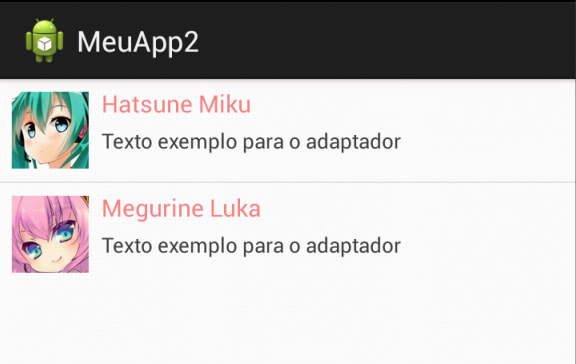
\includegraphics[width=.475\textwidth]{figuras/design/lista-composta.png}
  \caption{Lista Composta}
  \label{fig:e}
\end{figure}

%%% EXPANDABLE LIST %%%
\section{Listas expandíveis \texttt{(ExpandableListView)}}

Listas expandíveis são úteis para agrupar conjuntos de itens semelhantes, funcionam da mesma maneira que as listas comuns e podem ser customizadas.
Comece colocando sua lista na \emph{activity} desejada.
	
\begin{listing}[H]
\inputminted[linenos=true,fontsize=\small,frame=lines, framesep=2mm, tabsize=2,numbersep=5pt]{xml}{src/design/exlist.xml}
\caption{Lista expandível no \texttt{activity\_main.xml}}
\end{listing}	

O atributo \texttt{android:transcriptMode=''alwaysScroll'}' vai fazer com que a lista sempre role até o final quando você expande ou contrai um grupo.
 
Agora crie 2 novos arquivos XML, um chamado \texttt{list\_item\_parent.xml} e o outro chamado \texttt{list-item-child.xml}

\begin{listing}[H]
\inputminted[linenos=true,fontsize=\small,frame=lines, framesep=2mm, tabsize=2,numbersep=5pt]{xml}{src/design/list-item-parent.xml}
\caption{Layout \texttt{list\_item\_parent.xml}}
\end{listing}	

\begin{listing}[H]
\inputminted[linenos=true,fontsize=\small,frame=lines, framesep=2mm, tabsize=2,numbersep=5pt]{xml}{src/design/list-item-child.xml}
\caption{Layout \texttt{list\_item\_child.xml}}
\end{listing}	

Agora crie uma classe para o pai dos grupos chamada \emph{Parent}, que será responsável apenas por conter os dados do pai e os objetos filhos.

\begin{listing}[H]
\inputminted[linenos=true,fontsize=\small,frame=lines, framesep=2mm, tabsize=2,numbersep=5pt]{java}{src/design/parent.java}
\caption{Classe \texttt{Parent}}
\end{listing}	

\newpage

Crie uma nova classe, \texttt{CustomAdapter} que será o adaptador da lista expandível para os dados, para esse exemplo estaremos adaptando apenas para o uso de \emph{strings}.
Essa classe deve extender a classe \texttt{BaseExpandableListAdapter} 

\inputminted[linenos=true,fontsize=\small,frame=lines, framesep=2mm, tabsize=2,numbersep=5pt]{java}{src/design/customadapter.java}
\captionof{listing}{Classe \texttt{CustomAdapter}}


Para finalizar, você deve construir os objetos na classe da \emph{activity}, nesse exemplo para popular a lista eu coloquei no arquivo de \texttt{strings} alguns fabricantes e modelos de carros, você pode obtê-los no repositório do projeto.

\begin{listing}[H]
\inputminted[linenos=true,fontsize=\small,frame=lines, framesep=2mm, tabsize=2,numbersep=5pt]{java}{src/design/exlist-main.java}
\caption{Construindo a lista expandível na \emph{activity}}
\end{listing}	

\begin{figure}[H]
  \centering
  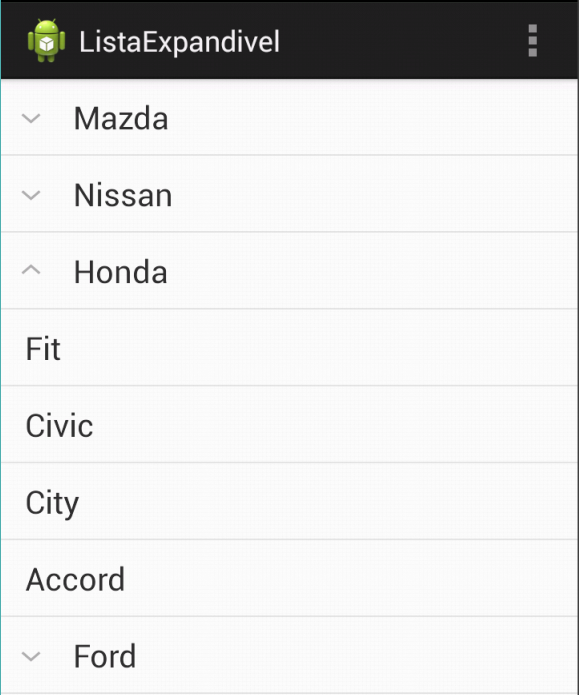
\includegraphics[width=.475\textwidth]{figuras/design/listaexpandivel.png}
  \caption{Exemplo de lista expandível}
  \label{fig:e}
\end{figure}

%%% GRADES E IMAGENS %%%

\section{Grades \texttt{(GridView)} e imagens \texttt{ImageView}}

Grades são úteis para mostrar imagens e fotos como uma galeria, ou permitir a seleção de categorias semelhante a uma lista. A idéia é ter elementos lado a lado para mostrar ou para selecionar e mostrar mais detalhes. Basicamente funciona como uma grade bi-dimensional que pode ser arrastada para os lados ou de cima pra baixo. 

\begin{figure}[H]
  \centering
  
\includegraphics[width=.475\textwidth]{figuras/design/gridview.png}
  \caption{Esquema de um \texttt{Grid view}}
  \label{fig:e}
\end{figure}

\newpage 
Comece por simplesmente colocando um layout \texttt{grid view} em sua activity.

\begin{listing}[H]
\inputminted[linenos=true,fontsize=\small,frame=lines, framesep=2mm, tabsize=2,numbersep=5pt]{xml}{src/design/gridview.xml}
\caption{Layout do \texttt{Grid View}}
\end{listing}	
\newpage
Crie uma nova classe que vai ser o adaptador para mostrar a imagem na grade, lembre-se que você pode adaptar qualquer layout para uma grade. Chame essa classe de \texttt{ImageAdapter}

\begin{listing}[H]
\inputminted[linenos=true,fontsize=\small,frame=lines, framesep=2mm, tabsize=2,numbersep=5pt]{java}{src/design/imageadapter.java}
\caption{Classe \texttt{ImageAdapter}}
\end{listing}	

Agora basta criar na grade na sua \emph{activity}.

\begin{listing}[H]
\inputminted[linenos=true,fontsize=\small,frame=lines, framesep=2mm, tabsize=2,numbersep=5pt]{java}{src/design/grade-activity.java}
\caption{\emph{activity} com grade}
\end{listing}	

Exemplo rodando:

\begin{figure}[H]
  \centering
  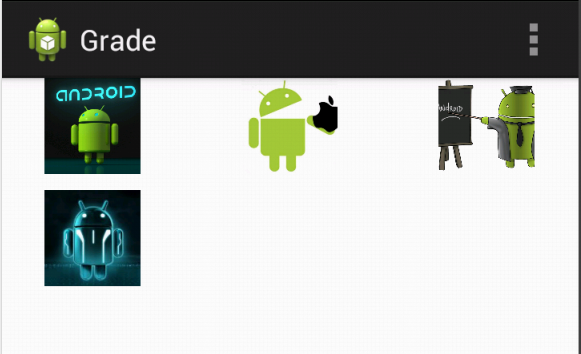
\includegraphics[width=.475\textwidth]{figuras/design/grade-exemplo1.png}
  \caption{Demonstração de um \texttt{Grid view}}
  \label{fig:e}
\end{figure}

Para complementar, você pode fazer com que a imagem abra em tela cheia quando clicada na view, para isso é necessário que você passe o \emph{id} do recurso do \texttt{GridView} para a nova \emph{activity}.
Crie um novo XML e chame de \texttt{full\_image.xml}, nele teremos apenas um \texttt{ImageView}.

\begin{listing}[H]
\inputminted[linenos=true,fontsize=\small,frame=lines, framesep=2mm, tabsize=2,numbersep=5pt]{xml}{src/design/full-image.xml}
\caption{Layout \texttt{full\_image.xml}}
\end{listing}	

Em seguida, crie uma nova classe chamada \texttt{FullImageActivity}, essa é \emph{activity} que vai mostrar a imagem em tela cheia. A construção da classe é simples, você deve apenas obter o \emph{id} da imagem passado como \emph{extra} através do \texttt{intent} e então obter essa imagem da classe \texttt{ImageAdapter}.

\begin{listing}[H]
\inputminted[linenos=true,fontsize=\small,frame=lines, framesep=2mm, tabsize=2,numbersep=5pt]{java}{src/design/FullImageActivity.java}
\caption{Classe \texttt{FullImageActivity}}
\end{listing}	 	 	

Finalmente, você deve modificar a \emph{activity} da sua grade para suportar o novo comportamento, para isso é necessário configurar o \texttt{gridview} para tomar algumas ações quando um elemento da tela for clicado. Observe o código que deve ser adicionado da sua \emph{activity}.

\begin{listing}[H]
\inputminted[linenos=true,fontsize=\small,frame=lines, framesep=2mm, tabsize=2,numbersep=5pt]{java}{src/design/grid-activity-p2.java}
\caption{\emph{activity} com grade, melhorado}
\end{listing}	 

Na linha 14 você pode observar a criação de um \emph{listener} para os itens clicados da grade, o método \texttt{onItemClick()} permite obter algumas informações sobre o item clicado e você pode usar essas informações como quiser, nesse caso é colocado dentro de um \texttt{intent} o \emph{id} do item clicado como sendo sua posição nessa grade. Finalmente o método \texttt{startActivity} é chamado e passando o \texttt{intent} criado como parâmetro.   

%% FRAGMENTOS %%
\section{Fragmentos}

Fragmentos são a solução do Android para criar interfaces de usuário modulares, eles vivem dentro das \emph{activity} e uma \emph{activity} pode conter vários fragmentos. Assim como as \emph{activity} os fragmentos possuem um ciclo de vida %% EXPLICAR MELHOR %%.
Dentre as vantagens de um fragmento estão:
\bi
	\item Modularidade e reuso de código
	\item Habilidade de construir interfaces com múltiplos painéis
	\item Facilidade de construir aplicativos para celulares e tablets
\ei

O primeiro conceito a ser coberto é como construir um fragmento, comece definindo o \emph{layout} do fragmento.

Um layout bem simples, apenas com um botão para efeito de demonstração. Agora crie uma classe \texttt{BasicFragment}

\begin{listing}[H]
\inputminted[linenos=true,fontsize=\small,frame=lines, framesep=2mm, tabsize=2,numbersep=5pt]{java}{src/design/basicfragment.java}
\caption{Classe \texttt{BasicFragment}}
\end{listing}	

Caso você esteja desenvolvendo para API menores que 11 (HoneyComb 3.0) você vai precisar usar a API de retrocompatibilidade que o Google providenciou para essas APIs, você precisa importar a classe de suporte: \mint{java}|import android.support.v4.app.Fragment;|

%% diferença chave? %%
% One of the key differences between a Fragment and an Activity is that Fragments instantiate their Views inside the onCreateView() callback and Activities instantiate their Views using the setContentView() method inside of the onCreate() callback. Fragments also have to manually instantiate their Views using an instance of LayoutInflater, which is provided to the onCreateView() method for convenience. %%

%% Another difference is that a Fragment is not a subclass of Context. This means that a Fragment can not be launched as a component inside your app and therefore always has to live inside of an Activity. This also means that whenever you need a Context inside of a Fragment, you need to get access to the parent Activity. You can do this by using the getActivity() method as we have done in the Fragment button's OnClickListener callback. You need to watch out because getActivity() can return null depending on where the Fragment is in the Activity's lifecycle. So, you should also include a check to see if the Activity is null before you use it. %%

Agora para incluir o fragmento na \emph{activity} existem duas opções. A primeira é inlcuir o fragmento no XML da \emph{activity} como você faria com qualquer \texttt{view}.

\begin{listing}[H]
\inputminted[linenos=true,fontsize=\small,frame=lines, framesep=2mm, tabsize=2,numbersep=5pt]{xml}{src/design/fragment-activity.xml}
\caption{Layout da \emph{activity} com um fragmento}
\end{listing}	

Você pode usar o \texttt{<fragment>} quantas vezes quiser para incluir múltiplos fragmentos.
Note que você precisa usar um nome qualificado em \texttt{android:name}, veja mais na documentação oficial: \href{http://developer.android.com/guide/topics/manifest/activity-element.html\#nm}{activity-element}\footnote{\href{http://developer.android.com/guide/topics/manifest/activity-element.html\#nm}{http://developer.android.com/guide/topics/manifest/activity-element.html\#nm}}

Novamente, caso esteja desenvolvendo para APIs menores que 11, você vai precisar fazer a \emph{activity} extender a classe \texttt{FragmentActivity} e importar a classe de suporte: \mint{java}|import android.support.v4.app.FragmentActivity;|
\mint{java}|public class MainActivity extends FragmentActivity|


Simplesmente configurando a \emph{activity} para usar o fragmento vai fazer com que o fragmento seja adicionado e renderizado na tela, entretanto você deve querer ter mais controle de quando e como seus fragmentos serão adicionados durante o curso do seu aplicativo. Para isso existe uma maneira alternativa de adicionar o fragmento em tempo de execução. A fim de adicionar o fragmento em tempo de execução você precisa fazer uma mudança no layout da \emph{activity}:

\begin{listing}[H]
\inputminted[linenos=true,fontsize=\small,frame=lines, framesep=2mm, tabsize=2,numbersep=5pt]{xml}{src/design/framelayout.xml}
\caption{Layout da \emph{activity} com o \texttt{FrameLayout}}
\end{listing}	

E uma mudança na \emph{activity} que vai mostrar o fragmento:

\begin{listing}[H]
\inputminted[linenos=true,fontsize=\small,frame=lines, framesep=2mm, tabsize=2,numbersep=5pt]{java}{src/design/activity-frag-dyn.java}
\caption{\emph{activity} com adição dinâmica de fragmento}
\end{listing}	

E dessa forma obtemos o mesmo resultado, porém com a adição dinâmica do fragmento, você pode experimentar e fazer com que o botão remova um fragmento e coloca outro diferente no lugar.

%% TABS %%

\section{Abas (\emph{Tabs})}
	Existem diversas maneiras de criar uma interface com abas no Android, uma delas é usando as interfaces \texttt{TabHost} e \texttt{TabWidget}, outra é imitando o comportamento usando apenas \texttt{Fragments}. 

	%% TABHOST TABWIDGET %%	
	\subsection{Usando \texttt{TabHost} e \texttt{TabWidget}}
	
	Abas usando essas interfaces são suportados pro todas as versões do android	
	Vamos criar uma interface com abas seguindo esse esquema:
	
	\begin{figure}[H]
	  \centering
	  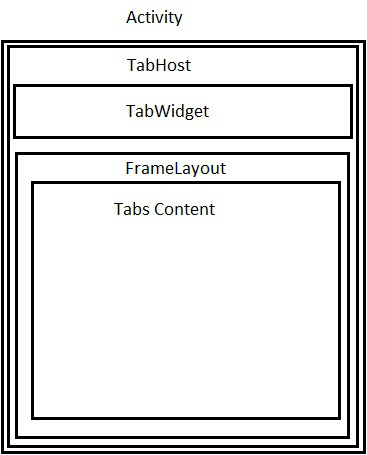
\includegraphics[width=.475\textwidth]{figuras/design/tabs1.jpg}
	  \caption{Esquema da interface com abas}
	  \label{fig:e}
	\end{figure}
	
	
	
	
	
	
	
\section{Arrastar \texttt{(SwipeView)} com abas}
\section{Menu lateral}


\end{singlespace}



%%%%%%%%%%%%%%%%%%%%%%%%%%%%%%%%%%%%%%%%%%%%%%%%%%%%%%%%%%%%%%%%%%%%%%%%%%%%%%%%

\singlespace
\selectlanguage{brazil}
\cleardoublepage
\thispagestyle{empty}
\phantomsection
\doublespace


\appendix
\addtocontents{toc}{\protect\setcounter{tocdepth}{0}} % as seções do apêndice não aparecem do sumário com este comando...
%%%%%%%%%%%%%%%%%%%%%%%%%%%%%%%%%%%%%%%%%%%%%%%%%%%%%%%%%%%%%%%%%%%%%%%%%%%%%%%%
\ape{apen}{Especificação blá, blá, blá}

Isto é um apêndice...

%%%%%%%%%%%%%%%%%%%%%%%%%%%%%%%%%%%%%%%%%%%%%%%%%%%%%%%%%%%%%%%%%%%%%%%%%%%%%%%%
\addtocontents{toc}{\protect\setcounter{tocdepth}{1}}

\end{document}
